\section{Selection Process} 

About the 4 techniques..

\subsection{Triangulation} %stefan
\subsubsection*{Summary}
Since our plant has a specified size in which the location of multiple objects has to be performed the method of Triangulation is one promising technic in which research was made. 
Triangulation was already a common principle of measurement in the 18th century and it´s divided between active and passive triangulation. Passive triangulation is a geometrical method based on two measurement stations which positions are known exactly. At these two measurement points angels of the desired point in space are measured to compute the localization in the specified coordinate system (x, y, z) with trigonometrical formulas.
With respect to the two measurement points which were already used in the 18th century nowadays two cameras are installed to perform a geographical method of 3D object-data estimation fig. \ref{Triangulation}.
\begin{figure}[!htbp]
\centering
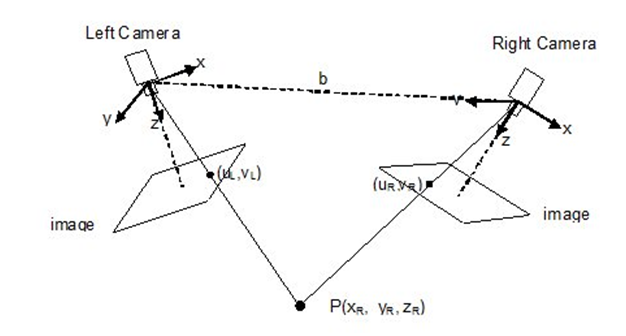
\includegraphics[width = 16cm]{Pictures/Triangulation}
\caption{Passive Triangulation set-up with two cameras}
\label{Triangulation}
\end{figure}\\
To Solve the problem, it is necessary to know the parameters of the left and the right camera visualized in the figure. In theory the triangulation is trivial, since each and every point of the images of the respective cameras maps to a line in 3D space. If a pair of corresponding points, in the case of the pipes less plant it would be an AGV, is found the projection of a point x in 3D space can be computed. 
Active triangulation in comparison to passive triangulation needs one camera and at least one source of structured light (e.g. Laser). As the passive way here the geometrical location and orientation of the camera and light source is space need to be known. Two possible set-ups with either a laser point and a stripe as structured light are shown in fig. \ref{ative_Triangulation}.
\begin{figure}[!htbp]
\centering
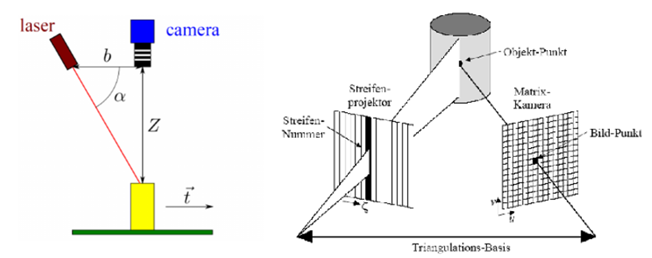
\includegraphics[width = 16cm]{Pictures/acticetriangulation}
\caption{Active Triangulation}
\label{ative_Triangulation}
\end{figure}\\
To solve the active triangulation problem, the structured light has to point on object which location is desired to estimate, in the case of the pipe less plant it would be the AGV. If this point is found on the 2D image of the camera, a triangulation with basic trigonometrical formulas which are using the properties and parameters of the camera and light source can be performed and the position of the AGV is estimated. 
\subsubsection*{Implementation} 
One possible way to implement a solution for the passive triangulation is to attach 2 high resolution cameras with USB 3.0 for a fast data transmitting on two edges of the plant being not on each others opposite side as shown in fig. \ref{ ative_Triangulation_implementation}.
\begin{figure}[!htbp]
\centering
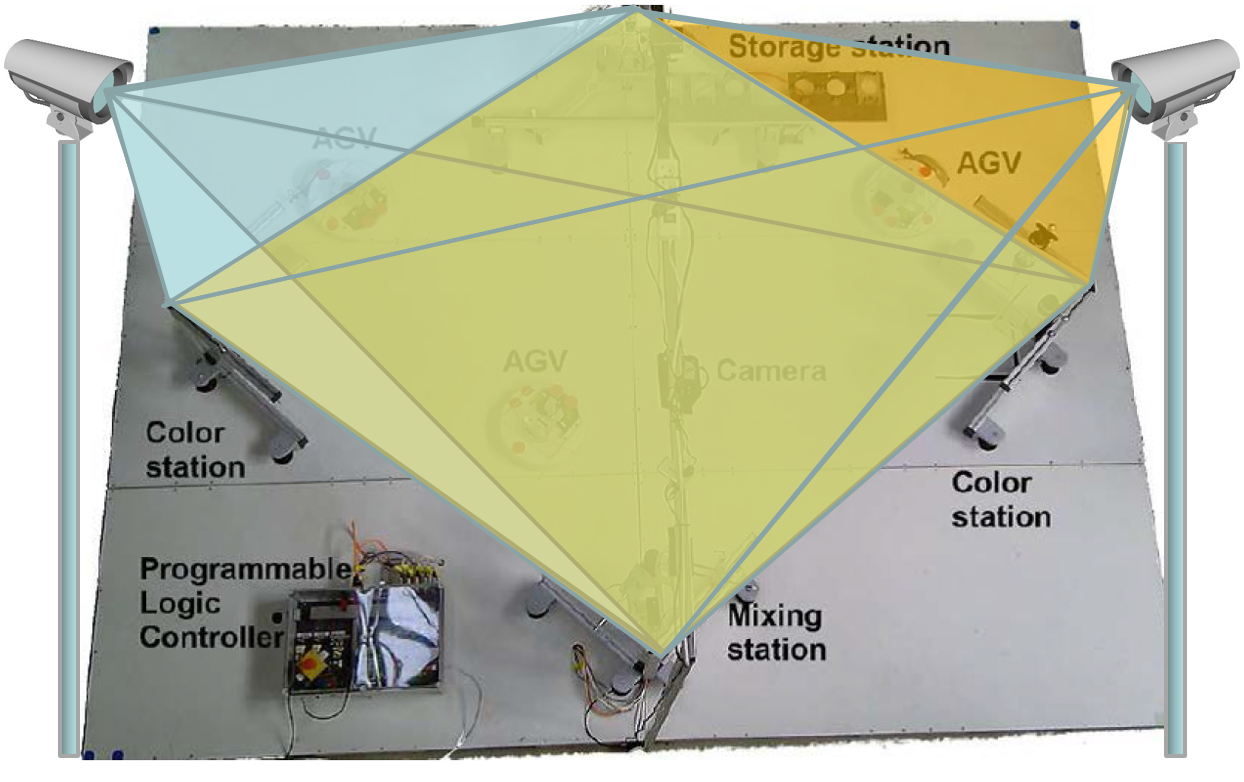
\includegraphics[width = 16cm]{Pictures/triangulationimplementatio}
\caption{Impmentation of passive triangulation}
\label{ative_Triangulation_implementation}
\end{figure}\\
The left and right camera are sequentially taking pictures which are transmitted to the plants computer where the image processing takes place. 

\subsubsection*{Pro and con}
\begin{table}[]
\centering
\begin{tabular}{|l|l|}
\hline
\multicolumn{2}{|c|}{\textbf{Passive Triangulation}}                                                                                                                  \\ \hline
\multicolumn{1}{|c|}{\textbf{Positive}}                                                                                    & \multicolumn{1}{c|}{\textbf{Negative}}   \\ \hline
Upgrade to USB 3.0 for faster data transmitting possible                                                                   & Light dependent                          \\ \hline
\begin{tabular}[c]{@{}l@{}}Upgrade to a camera with higher resolution to reduce \\ measurement error possible\end{tabular} & New concept of orientation may be needed \\ \hline
No Fish-Eye-Lense problem                                                                                                  & Limited range of observation             \\ \hline
Low cost                                                                                                                   &                                          \\ \hline
                                                                                                                           &                                          \\ \hline
\end{tabular}
\caption{Positive and Negative Points of Passive Triangulation}
\label{pro_con_passive_tri}
\end{table}
\begin{table}[]
\centering
\begin{tabular}{|l|l|}
\hline
\multicolumn{2}{|c|}{\textbf{Active Triangulation}}                                                                                                                     \\ \hline
\multicolumn{1}{|c|}{\textbf{Positive}}                                                                                    & \multicolumn{1}{c|}{\textbf{Negative}}     \\ \hline
Upgrade to USB 3.0 for faster data transmitting possible                                                                   & New unknown laser technology is needed     \\ \hline
\begin{tabular}[c]{@{}l@{}}Upgrade to a camera with higher resolution to reduce \\ measurement error possible\end{tabular} & High costs for several Laser (one per AGV) \\ \hline
Easy detection of laser points on camera image                                                                             & Laser needs to move while AGVs are moving  \\ \hline
                                                                                                                           & Limited range of observation               \\ \hline
                                                                                                                           & Light dependent                            \\ \hline
\end{tabular}
\caption{Positive and Negative Points of Active Triangulation}
\label{pro_con_active_tri}
\end{table}



\subsection{Pattern Recognition} %medhini
\subsubsection*{Summary} 
\subsubsection*{Implementation}
\subsubsection*{Pro and con}
..

\subsection{RFID} % stephan
\subsubsection*{Summary} 
\subsubsection*{Implementation}
\subsubsection*{Pro and con}
..

\subsection{Map-Based Localization} %abdul
\subsubsection*{Summary} 
\subsubsection*{Implementation}
\subsubsection*{Pro and con}
..



example:
\begin{table}[h!]
\centering
 \begin{tabular}{||c c c c||} 
 \hline
 Col1 & Col2 & Col2 & Col3 \\ [0.5ex] 
 \hline\hline
 1 & 6 & 87837 & 787 \\ 
 2 & 7 & 78 & 5415 \\
 3 & 545 & 778 & 7507 \\
 4 & 545 & 18744 & 7560 \\
 5 & 88 & 788 & 6344 \\ [1ex] 
 \hline
 \end{tabular}
 \caption {Should be a caption}
\end{table}
